\graphicspath{ {mainmatter/Magnusson_2007/} }

\title*{2007: The Acoustic, the Digital and the Body: A Survey on Musical Instruments}
\titlerunning{A Survey on Musical Instruments}

\author{Thor Magnusson and Enrike Hurtado}
\authorrunning{Magnusson and Hurtado}

%\institute{Thor Magnusson \at Department of Music, University of Sussex,  Brighton, United Kingdom, \email{t.magnusson@sussex.ac.uk}
%\and Enrike Hurtado  \at Department of Art and Technology, EHU/UPV University of the Basque Country, Leioa, Bizkaia. Spain,\email{enrike@ixi-software.net}
%}
%
%
\maketitle
%\blfootnote{Original affiliations: Thor Magnusson: Creative Systems Lab, University of Sussex. Enrike Hurtado : Digital Research Unit, University of
%Huddersfield, Huddersfield, UK.}

\abstract*{This paper reports on a survey conducted in the autumn of 2006 with the
objective to understand people's relationship with their musical tools. The
survey focused on the question of embodiment and its different modalities in the
fields of acoustic and digital instruments. The questions of control,
instrumental entropy, limitations and creativity were addressed in relation to
the activities of playing, creating, or modifying instruments. The survey focus
was phenomenological, i.e., we were concerned with the \textit{experience} of
playing, composing for and designing digital or acoustic instruments. At the time
of analysis, we had 209 replies from musicians, composers, engineers, designers,
artists and others interested in this topic. The survey was mainly aimed at
instrumentalists and people who create their own instruments or compositions in
flexible audio programming environments such as SuperCollider, Pure Data, ChucK,
Max/MSP, CSound, etc.}

\section{Introduction}
For over six years we at ixi software \cite{Magnusson:2005,Magnusson:2006} have been creating alternative
instruments for the computer, focusing on the graphical user interface and its
deterministic nature. We have tried to resist the temptation of imitating the
world of acoustic instruments or physical hardware. The goal has been to create
instruments that make effective use of the specific qualities of the computer
itself with its various hardware interfaces, but concentrating particularly on
the semiotic affordances of the screen as the main control interface.

We have created various instruments and software suites that are freely
available on our website. We also run a mailing list, a net label and we give
workshops in audio-visual programming at various universities and art
institutions all over Europe. Although we have had good and instructive feedback
from ixi software users, musical collaborators, and workshop participants, we
have been interested in developing a more systematic feedback or dialog, which
induced an interest in creating an online user survey, addressing the questions
we focus on in our work.

In the survey we were specifically concerned with people's experience of the
difference between playing an acoustic and a digital instrument. The approach was
phenomenological and qualitative: we wanted to know how musicians and composers
describe the practice and relationship with their musical tools, whether acoustic
or digital. We deliberately did not define what we meant by ``digital
instrument'' (such as sequencer software, graphical dataflow language, textual
programming language or sensor interfaces mapped to sound),\footnote{For a
discussion of the taxonomy of screen-based instruments or composing environments,
see Duignan, Noble and Biddle \cite{Duignan:2005}. Although the authors mainly focus on
sequencing tools (and they acknowledge that they have a broad definition of the
term) the taxonomy is still valid here in this context.} as we were interested
in how people \textit{themselves} define the digital, the acoustic, and the
relationship between the two. How do people rate the distinctive affordances and
constraints of these instruments and is there a difference in the way they
critically respond to their design? Furthermore, do people relate differently to
the \textit{makers} of these two types of instruments? We were also curious to
learn whether musical education and a history of practicing an acoustic
instrument yields a different critical relationship to the digital instrument.
How does instrumental practice change the ideas of embodiment and does it affect
the view of the qualitative properties of the computer-based tool? Finally, we
were interested in knowing how people relate to the chaotic or
``non-deterministic'' nature of their instruments (if they see it as a limitation
or a creative potential) and whether they feel that such ``quality'' could be
arbitrarily\footnote{Arbitrarily, as everything has to be programmed into the
digital instruments vs. the fact that acoustic instruments always contain those
properties already due to their materiality.} designed into digital instruments.


In order to gain a better understanding of these questions and the basis for
people's views, we also asked the participants about their background in working
with the computer; which operating systems they run; what software they
predominantly use and the reasons they have chosen that environment for their
work.

\section{The Survey}

\subsection{The Participants}
The group we tried to reach to with our survey was very wide, i.e., from the
acoustic instrumentalist that has never used a computer for music to the live
coder who might not play a traditional instrument. More specifically we were
interested in learning about people who have a critical relationship with their
tools (whether acoustic or digital) and build their own or modify existing
instruments, to allow for their preferred way of expressing themselves musically.
We were also curious to hear from people who have used our software how they
experience ixi software in relation to the questions described above.

The results we got were precisely from the group we focused on. The majority of
the participants actively work with one or more of the audio programming
environments that we asked about. There were very few replies from people who use
exclusively commercial software such as Cubase, ProTools or Logic.

\begin{figure}[t]
\centering
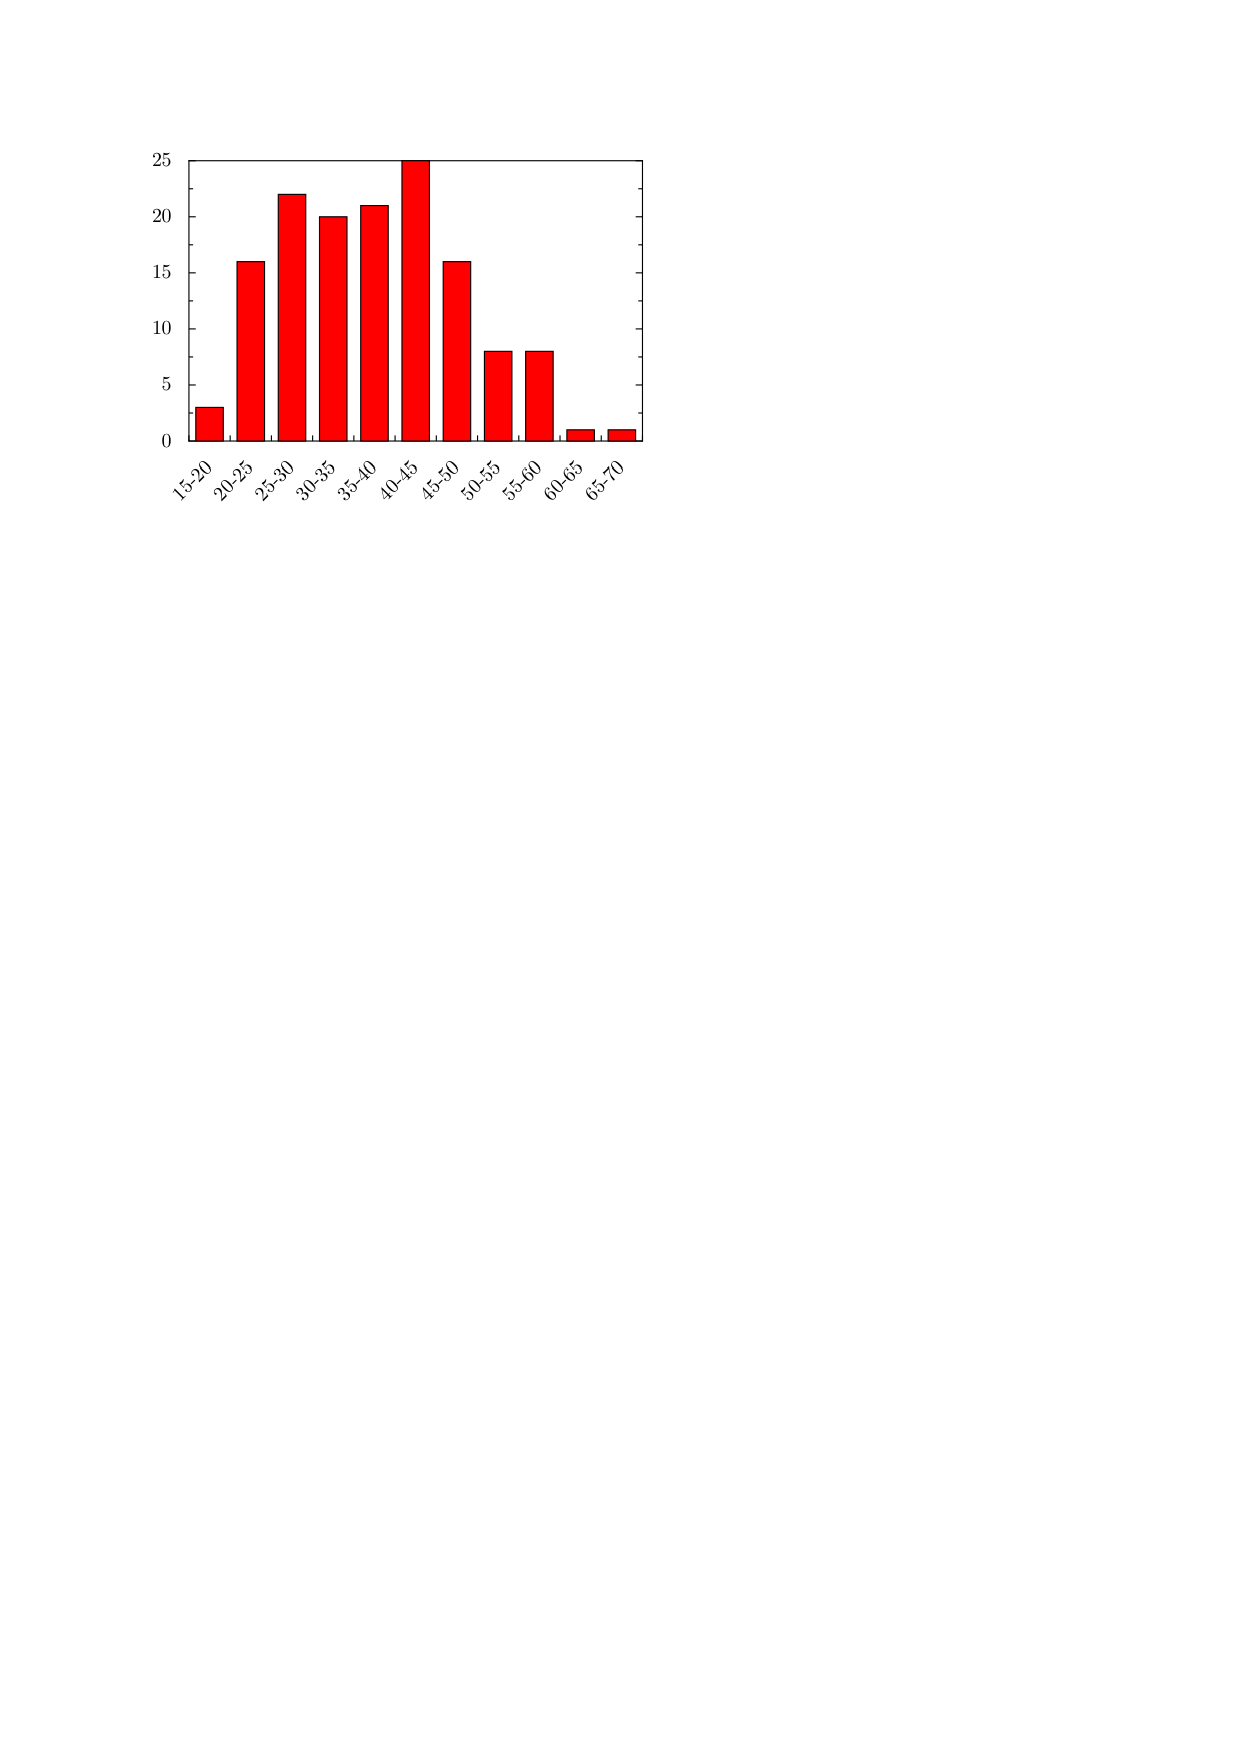
\includegraphics[width=240pt]{img-1-eps-converted-to.pdf}
\caption{The age distribution of the survey participants. The Y axis
shows number of participants; X axis the age-range.}
\label{Magnusson:fig:1} 
\end{figure}

The survey had 209 replies, mainly from Western Europe and North America, but a
considerable amount also from South America and Asia. Of all the replies there
were only 9 female participants, which is a frustrating state of affairs, but it
is outside the scope of this survey and research to explore the reason behind
this fact. However, we were interested in the age of the participants and how
long they have been playing music. We were surprised how relatively high the mean
age was (37 years), distributed as shown in Figure~\ref{Magnusson:fig:1}.

\subsection{The Questionnaire}

The survey was qualitative, where the main focus was on people's description of
their musical tools. It was divided into six areas:

\begin{enumerate}
\item \textbf{Personal Details}: a set of demographic questions on gender, age,
profession, nationality, institutional affiliation, etc.

\item \textbf{Musical Background}: questions on how the participants defined
themselves in relation to the survey (musician, composer, designer, engineer,
artist, other), how long they had played music, musical education, computer use
in music and musical genre (if applicable).

\item \textbf{Acoustic Instruments}: questions about people's relationship with
their instrument. (Which instrument, how long they have played it, etc.). We
asked whether people found their instrument lacking in functionality; if they
thought the instrument has ``unstable'' or ``non-deterministic'' behaviour; and
if so, how they relate to that. We asked how well they knew the history of their
instrument and which factors affected the design of it. And we posed the maverick
question: would it be beneficial if the human body was different?

\item \textbf{Digital Instruments}: we asked which operating system people use and
why; what hardware (computer, soundcard, controllers, sensors); what music
software; and whether they have tried or use regularly the following audio
programming environments: Pure Data, SuperCollider, ChucK, CSound, Max/MSP,
Plogue Bidule, Aura, Open Sound World, AudioMulch and Reaktor. We asked about
their programming experience and why they had chosen their software of choice.
Further, we were interested in knowing if and how people use the Open Sound
Control (OSC) and whether people use programming environments for graphics or
video in the context of their music making.

\item \textbf{Comparison of Acoustic and Digital Instruments}: here we were
concerned with the difference of playing acoustic and digital instruments, and
what each of the types lack or provide. We asked about people's dream software;
what kind of interfaces people would like to use; and then if people found that
the limitations of instruments are a source of frustration or inspiration. Did
that depend on the type of instrument?

\item \textbf{ixi software}: this section of the questionnaire is only indirectly
related to this paper. Here we wanted to know when and where the participants
came across ixi software, how they use the software and which applications they
use. We asked if there are characteristics in the design of the software that
goes across the different applications and if these characteristics are
signatures that influence the musical outcome. We were interested if people found
they are free or limited in the use of ixi software. Is the graphical element (in
the style that we use in ixi software) a positive or a negative feature?
\end{enumerate}

People were free to answer the questions they were interested in and to skip the
others, as it would not make sense to force an instrumentalist to answer
questions about computers if he/she has never used one. The same goes for the
audio programmer that does not play an acoustic instrument. For people interested
in the questions, the survey can still be found online.\footnote{\url{http://www.ixi-software.net/survey}}

\subsection{The Methodology}
The survey was introduced on our website and we posted it to the ixi mailing
list, but we also sent it to various external mailing lists (including
SuperCollider, ChucK, Pure Data, Max/MSP, CSound, AudioMulch, eu-gene, livecode)
and asked friends and collaborators to distribute the survey as much as possible.
We contacted orchestras and conservatories and asked them to post the survey on
their internal mailing lists. The survey could be answered in 9 languages, but
the questions themselves were only available in English or Spanish.
Unfortunately, as around quarter of the visitors on our website are from Japan,
where there is a strong culture in the use of audio programming languages, we did
not have the resources to translate the survey into Japanese.

After three months of receiving replies, we started parsing the data. We
analysed each reply and put it into a database. All the quantitative data was
filled in quickly, but as the questionnaire was largely qualitative (where people
write their answers in the form of descriptive narrative), we had to interpret
some of the data subjectively. Here we created a bipolar continuum (marked from 1
to 5) where the following ``archetypal'' elements were extracted: a) abstract vs.
graphical thinking: i.e., the tendency for working with textual vs. dataflow
programming environments. b) preference of self-made vs. pre-made tools. c)
embodied vs. disembodied emphasis in playing and making instruments or
compositions d) whether the person is a ``techie'' vs. ``non-techie'' where we
tried to extract the level of people's ``computer-literacy'' and programming
skills, e) academic vs. non-academic. We were interested in the question of how
these audio programming environments (that mostly have their origins in academia)
have filtered out into the mainstream culture.

\begin{figure}[t]
\centering
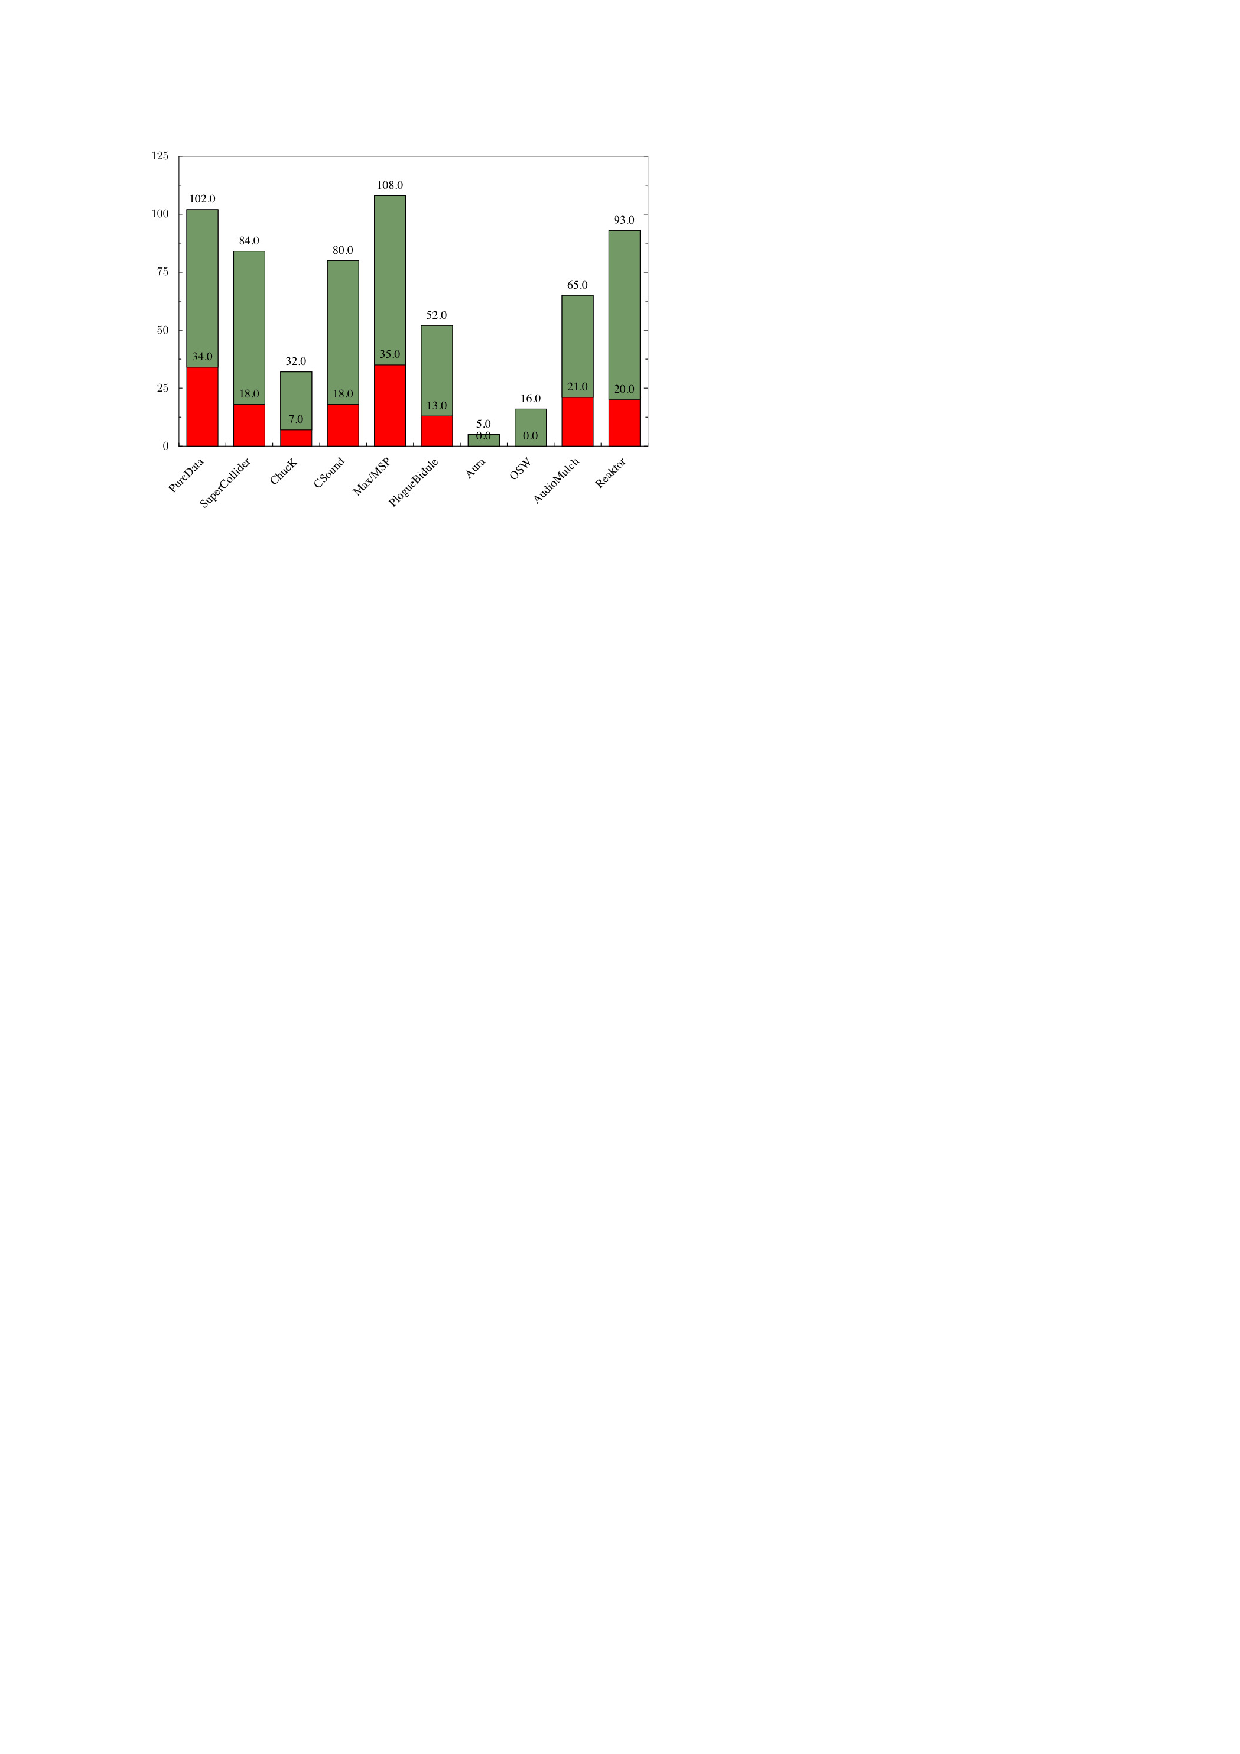
\includegraphics[width=\textwidth]{img-2-eps-converted-to.pdf}
\caption{Tool-usage of the survey participants. The higher number shows
how many people use or have used the specific tool. The lower number shows their
tool of choice.}
\label{Magnusson:fig:2} 
\end{figure}

The continuum we used for marking this had values from 1 to 5 with ``nil'' as a
valid entry where it was impossible to extract any meaningful value from the
answers. In order to test how reliable this subjective method of categorising the
answers was, we selected five random replies and gave the same set of replies to
five external peers to analyse. The results were almost identical, with some
minor differences on the left or right side of the continuum; but never opposite
interpretations.

\section{The Evaluation}
There were many questions in our survey that addressed the issues of acoustic
vs. digital instruments from different angles but they were varied approaches or
``interfaces'' to some underlying topics of interest. In the next sections we
will look at some selected topics and what we learned from the answers.

\subsection{The Survey Participant}
From analysing the demographic of the people answering the survey, we could
divide the typical survey participant into two groups of which more than 90
percent of the participants would belong: a) People who have had over 20 years of
studying music and playing acoustic instruments, therefore typically 30-40 years
of age or older. They have been using the computer for their music for at least
10 years and usually have some form of programming experience. Many write their
own software or use the common audio programming environments available today.
This group has thought a lot about their instruments and why they have chosen to
work on their music using the computer. b) The other group consists of younger
people who grew up with the computer and are also highly computer literate. Many
of them had not received formal musical education nor practiced on an acoustic
instrument, but use the computer as their instrument and environment for creating
music. Here, of course, we could view the time spent in front of the computer
screen performing any task as part of the musical training. Naturally there was
some degree of overlap between the two groups.

It might be illustrative to look at which operating systems the participants are
running their tools on, and here we see that 45 people use Linux/GNU; 105 use
Windows; and 88 use Mac OS. Of these 16 stated that they use both Mac OS and
Linux/GNU; 30 use both Mac OS and Windows; 25 Linux/GNU and Windows; and 7 used
all three. Other operating systems in use were NeXTstep, BSD and Solaris, one
person each system.

\subsection{Acoustic vs. Digital Instruments}
The question we were concerned with here is how people experience the different
qualities of acoustic instruments and digital instruments or software tools.
Apart from the experiential and perceptual differences, do people think that the
tools enframe or influence their work?

Many people found that an important difference in these two types of instruments
lies in the fact that the digital instrument can be created for specific needs
whereas the player has to ``mould oneself'' to the acoustic instrument. As the
composed digital instrument can be very work specific, it lacks the generality of
acoustic instruments. Related to this, some people reported discontent with the
uncertainty of the continuation of commercial digital instruments or software
environments. Their production could be discontinued or not supported on new
operating systems. Unless open source is used, the proprietary protocols could
render the instruments objects of archaeology. In this regard, acoustic
instruments have longer lifetime, which makes practising them more likely a
continuous path to mastery.

Some survey participants expressed the wish for more limited expressive software
instruments, i.e., not a software that tries to do it all but ``does one thing
well and not one hundred things badly.'' They would like to see software that has
an easy learning curve but incorporates deep potential for further explorations,
in order not to become bored with the instrument. True to form, the people asking
for such software tools had a relatively long history as instrumentalists.

Some participants expressed how they found their time better spent working with
digital technology, creating music or ``experimenting with sound,'' rather than
practicing an acoustic instrument. Conversely, others talked about the dangers of
getting side-tracked when using the computer, constantly looking for updates,
reading mailing lists, testing other people's patches or instruments, or ending
up browsing the web whilst trying to make music. Some talked about the
``frightening blank space'' of the audio programming patcher (meaning the endless
possibilities) and found retreat in limited tools or acoustic instruments,
whereas others were frustrated with the expressive limitations of the acoustic
instruments and craved for more freedom and open work environments. Naturally,
this went hand in hand with people's use of environments such as SuperCollider,
ChucK, Pure Data and Max/MSP vs. preference of less open or more directive
software like ProTools, Cubase, GarageBand, Fruityloops, etc.

Another issue of concern was latency. An acoustic instrument does not have
latency as such, although in some cases there is a delay between the energy
applied and the sounding result. In digital instruments there might be up to 50
ms. latency that people put up with when playing a hardware controller; many
seconds latency in networked performances; but also the organisational latency
when opening patches, changing effect settings or in live coding where one has to
type a whole function before hearing the result (typically by hitting the Enter
button). This artificial latency is characteristic of digital instruments, but
not necessarily a negative property except in the case of hardware controllers.


\begin{table}[t]
\centering
\ra{1.2}
\caption{Frequent comments on the positive and negative aspects of acoustic instruments.}
\vspace{3pt} \noindent
\begin{tabular}{ll}
\toprule
\textbf{Acoustic--Positive}     & \textbf{Acoustic--Negative}  \\
\midrule  
Tactile feedback		&		Lacking in range \\
Limitations inspiring		&		No editing out of mistakes \\
Traditions and legacy	&		No memory or intelligence \\
Musician reaches depth	&		Prone to clich\'e playing \\
Instrument becomes 2$^{nd}$ nature  \hspace{1cm} &	Too much tradition/history \\
Embodiment		&	No experimentation in design \\
No latency			&		Inflexible--no dialog \\
Easier to express mood		&	No microtonality or tunings \\
Extrovert state when playing	&	No inharmonic spectra \\
\bottomrule
\end{tabular}
\end{table}

The question of originality came up frequently. People found it possible to be
more original using the composed, digital instruments, precisely because of the
lack of history and traditions. As one survey participant put it: 

\begin{quotation}
when playing
an acoustic instrument, you are constantly referring to scales, styles,
conventions, traditions and clich\'{e}s that the instrument and the culture
around it imposes on you. A musician can just play those conventions in autopilot
without having to THINK at all. It's easy and unchallenging.
\end{quotation}

This, of course, is a double-edged sword, as it is difficult in a live performance using software tools to refer to the musical reservoir in the spur of the moment. All such decisions have to be pre-programmed and thus pre-planned. This issue of originality also points to the limited scopes of some commercial software environments where the users are almost led into producing music of certain styles.

People also discussed the problem of arbitrary mappings in digital
instruments \cite{Hunt:2002}. There are no ``natural'' mappings between the exertion of bodily
energy and the resulting sound. One participant described digital instruments as
``more of a mind/brain endeavour.'' He continued and stated that ``it is more
difficult to remove the brain and become one with the physical embodiment of
performing.'' Others described the perception of the vibrating physical object
and feeling of the source of the sound in their hands or on the body, as
something that computer systems lack with their plastic buttons and sliders,
soundcards and cables going out to speakers that are located far away from the
instrument played. Yet another participant talked about the enriching experience
of learning the vocabulary and voice of an instrument like the viola to its
finest details, whereas with computer technology the voice is too broad to get to
know it thoroughly.

\subsection{Affordances and Constraints}
Here we were interested in the question whether people relate differently to the
affordances and the limitations of their acoustic and digital instruments.

Responders commonly agreed that the limitations of acoustic instruments were sources of inspiration and creativity. People talked about ``pushing the boundaries'' of the instrument and exploring its limits. Many participants said the same about digital instruments, but more commonly people were critical of the limitations of software. Some felt that software limitations are due to engineering or software design, as opposed to the physical limitations of natural material like wood or strings. This fact makes people more critical of software tools than they are with acoustic instruments. There could be many reasons for this; one being that musical software is such a new field and naturally experimental whereas acoustic instruments have had centuries of refinement. Another observation that our data supports as well is that people normally start to learn an acoustic instrument at a very young age when things are more likely to be taken for granted. People see it as their fault if they cannot play the instrument properly, not the imperfection of the instrument design itself. This is different with digital instruments---at least with our survey participants---where people are more likely to criticise and see the limitations as weakness of the design rather than their own work methods or understanding of the system.

\begin{table}[t]
\centering
\ra{1.2}
\caption{Frequent comments on the positive and negative aspects of digital instruments.}
\vspace{3pt} \noindent
\begin{tabular}{ll}
\toprule
\textbf{Digital--Positive}     & \textbf{Digital--Negative}  \\
\midrule  
Free from musical traditions \hspace{1cm} & Lacking in substance  \\

Experimental--explorative & No legacy or continuation  \\

Any sound and any interface & No haptic feedback  \\

Designed for specific needs & Lacking social conventions  \\

Freedom in mapping & Latency frequently a problem  \\

Automation, intelligence & Disembodied experience  \\

Good for composing with & Slave of the historical/acoustic  \\

Easier to get into & Imitation of the acoustic  \\

Not as limited to tonal music & Introvert state when playing  \\
\bottomrule
\end{tabular}
\end{table}

Most of the skilled instrumentalists saw the limitations of their acoustic
instruments with positive eyes and viewed the potential---both discovered and
undiscovered---of the instrument as an expressive space in which they felt
comfortable. People usually had an ``emotional'' affection towards their acoustic
instrument (one of our questions asked about this) and they bonded with its
character. This issue is very different in regard to people's feelings about
their digital instruments. Survey participants often expressed frustrations with
the technology, irritating limitations of software environments and
dissatisfaction with how hardware needs constant upgrading, fixing and, not
surprisingly, the use of electricity. One responder talked about how the
limitations of acoustic instruments change or evolve constantly according to
skill levels but also state of mood, whereas the limitations of software, once it
has been learned and understood, are the limitations of the design. As another
participant put it: ``the creative challenge [in digital instruments] is to
select and refine rather than expand.''

In general people felt that the main power of digital instruments is that one
can design the instrument for specific needs. The process of designing the
instrument becomes a process of composing at the same time. The fact that people
talk about ``composing instruments'' \cite{Momeni:2005} indicates a clear distinction from the
acoustic world where instruments tend to be more general in order to be able to
play more varied pieces. This also explains why we rarely see the continuity of
digital instruments or interfaces through time: each instrument tends to be made
for a specific purpose. The power to be able to store conceptual structures in
the tool itself renders it more specific and unique for a certain musical piece
or performance and less adaptive for other situations. However, there is a
continuum where instruments are on the one side unique and specific and on the
other side general and multi-purpose. Creating a digital instrument always
involves decisions of where to place the instrument on that continuum.

\subsection{The Instrument Maker Criticised}
As discussed above, our survey shows that people have a different critical stance to the makers of acoustic and digital instruments (or software). This is reflected in the way people relate to the instruments themselves. The fact that acoustic instruments seem to have existed forever (and the survey shows that the majority of people do not have a very thorough historical knowledge of their instrument) makes people less likely to step back and actively criticise their instrument of choice.

Almost all the participants stated that their acoustic
instruments have been built from ergonomic and aesthetic/timbral considerations
and saw the evolution of their instrument as a refinement where it is moulded to
the human body. There is, however, evidence that orchestral instruments were
developed primarily with the view to stabilise intonation and augment acoustic
power or loudness \cite{Jorda:2005}. In fact, the young but strong tradition of digital music
instruments and interface building is perhaps more consciously concerned with
ergonomics and human-tool interaction than we find in the history of acoustic
instrument building. Ergonomics have at least become more prominent in the way
people think when building their musical tools. An agreed view was that the
difficulty of building masterly interfaces in the digital realm is largely
because of the complexity of the medium and the unnatural or arbitrary nature of
its input and output mappings.

In \textit{Being and Time} \cite{Heidegger:1995}, the philosopher Martin
Heidegger talks about two cognitive or phenomenological modalities in the way we
look at the world. In the first mode we have the usage of tools, where the tools
are \textit{ready-at-hand} and are applied in a finely orchestrated way by the
trained body. The second mode happens when the tool breaks and it becomes
\textit{present-at-hand}, i.e., the user of the tool has to actively think what
is wrong with the tool, and look at its mechanism from a new and critical stance.
Heidegger takes the example of a carpenter who uses the hammer day in and day out
without thinking about it. Only when the head falls off the hammer will the
carpenter look at the hammer from a different perspective and see it in its true
phenomenological light. As digital instruments/software are normally applied on
the computer, we are more likely to have these phenomenological breaks. The tool
becomes present-at-hand and we have to actively think about why something is not
working or what would be the best way of applying a specific tool for a certain
task. In fact, the way we use a computer and digital instruments is a constant
oscillation between these two modes of being ready-at-hand and present-at-hand.
We forget ourselves in working with the tool for a while, but suddenly we have to
open or save a file, retrieve a stored setting, switch between plug-ins or
instruments, zoom into some details, open a new window, shake the mouse to find
the cursor, plug in the power cable when the battery is low, kill a chat client
when a ``friend'' suddenly calls in the middle of a session, etc. In this
respect, many of the participants saw the computer as a distracting tool that
prevents the potential for deep concentration.

\subsection{Entropy and Control in Instruments}
Here we were interested in knowing how people relate to the non-deterministic
nature of their instruments and whether this differs in acoustic and digital
instruments.

We had two trends of responses here. It was mostly agreed that the accidental or
the entropic in acoustic instruments could be a source of joy and inspiration.
Some people talked about playing with the tension of going out on the ``slippery
ice'' where there was less control of the instrument. Typically people did not
have the same view of digital instruments. When they go wrong or unpredictable,
it is usually because of a bug or a fault in the way they are set up and most
people did not like that. However, there was a strand of people who enjoyed and
actively searched for such ``glitches'' in software, which of course has resulted
in the well known musical style called ``Glitch.''

Our data also illustrates how the process of exploration is a very common way of
working with software, where a system is designed in the form of a space of sonic
parameters, and the user navigates that space until a desired sound or musical
pattern is found.\footnote{For a discussion of compositional processes in
electronic music, see Eaglestone, Upton and Ford \cite{Eaglestone:2005}} This style of working is
quite common in generative music and in computationally creative software where
artificial intelligence is used to generate the material and the final fitness
function of the system tends to be the aesthetic judgement of the user.

\subsection{Time and Embodiment}
As most people would have guessed, we found that people who
had spent long hours practicing acoustic instruments emphasised the desire to
have physical control and use the body in a musical performance. Analysing our
embodied-disembodied continuous scale, we saw that the longer people had played
an acoustic instrument, the more they stressed the importance of embodiment in
their musical practice. Playing digital instruments seems to be less of an
embodied practice (where motor-memory has been established) as the mapping
between gesture and sound can be altered so easily by changing a variable, a
setting, a patch, or a program. Some responders noted that working with digital
instruments or software systems had forced them to re-evaluate the way they
understand and play their acoustic instrument. Of course, the contrary has to be
true as well.

There are a few things to note here. Most of the people who
answered the survey were both acoustic and digital instrumentalists and were
confident with the qualities of both worlds. It seems that people subscribe
positively to the qualities of each of the two instrumental modalities --
acoustic and digital---and do not try to impose working patterns that work in
one type instrument onto the other. In general people seem to approach each
instrument on its own merits and choose to spend time on it if it gives them some
challenge or excitement.

\section{Interesting Comments}

There were some comments that are worth printing here due to their direct and
clear presentation:

\begin{itemize}
\item ``I don't feel like I'm playing a digital instrument so much as operating it.''
\item ``Eternal upgrading makes me nervous.''
\item ``full control is not interesting for experimentation. but lack of control is not useful for composition.''
\item ``Can a software `instrument' really be considered an instrument, or is it something radically different?''
\item ``The relationship with my first instrument (guitar) is a love / hate one, as over the years I developed a lot of musical habits that are hard to get rid of ;-)''
\item ``j'entretiens un certain rapport avec mes machines. Impossible pour moi de penser \`{a} revendre une machine.''
\item ``I think acoustic instruments tend to be more right brain or spatial, and digital instruments tend to be more left brain and linguistic.''
\end{itemize}

\section{Discussion}
There were many surprising and interesting findings that came out of this
survey. First of all, we were surprised by the high mean age of the survey
participants. We wondered if the reason for the high average age could be the
nature of the questions, especially considering the questions regarding
embodiment. Perhaps the questions are not as relevant to the younger people who
have been brought up with the computer and are less alienated by the different
modes of physical vs. virtual interaction? A likely explanation is that the mean
age of the survey participants is reflecting that of the members of the mailing
lists we posted the survey to.

It is illustrative that the majority of people answering the survey were
involved with academia or had an academic or conservatory education. This helps
to explain the high mean age but also the high level of analysis that most people
had applied to their tools. We noted that the time spent playing an instrument
increases the focus on embodiment in players and as such the questions of this
survey might have connected better with the older musicians.

An important point to raise here is that whereas the survey focused on the
\textit{differences} of acoustic and digital instruments and people's perception
of those, the fact is that most people are content with working with both
instrumental modalities and subscribe to the different qualities of each when
using those specific tools. Many of the people answering the survey used the
computer in combination with acoustic instruments, especially for things that the
computer excels at such as musical analysis, adaptive effects, hyper-instruments
and artificial intelligence.

A clear polarity between the acoustic and digital instruments is the division
between an instrument maker and a musician/composer in acoustic instruments. In
the field of digital instruments, designing an instrument often overlaps with the
musical composition itself (or at least designing its conditions). There is a
continuum where people's work can be placed: from a personal expression in the
form of a composition to a software that can be distributed for others to use.

Another interesting trait we noticed in the survey was the question of open
source software. Many people are using Linux or expressing desire to do so
because they feel that they have more control over things and are less directed
by a specific company's ideas of how to set up the working environment or
compose/perform music. The questions of open protocols and standards, of legacy
in software, of collaborative design and freedom to change the system were all
important issues here.

\section{Future Work}
The topics of this survey revealed many more questions that would have been
inconceivable without the process of making this survey and studying the replies.
The next step in our research will be to perform interview sessions with both
acoustic and electronic musicians and laypeople. We would like to find out how
people experience graphical user interface design in musical software and whether
they think the functionality of the software represents or fits the mental model
they already have about how to compose and/or perform music. Can software be seen
as epistemic tools where acoustic instruments are more pragmatic tools?

\begin{acknowledgement}
Working on this survey has been immensely interesting and we would like to thank
all the participants for their efforts in answering the survey. Some of the
answers were profoundly intriguing, some gave nice twists in perspective and some
were incredibly witty. We would like to thank Nick Collins, Marcelo Wanderley,
Chris Thornton, Greg Hooper, Cian O'Connor, Tom Hall, Heimir Snorrason, Leire
Vergara, Birta Thrastardottir, Monica Guerrero and all the other people who were
involved in helping us with the survey.
\end{acknowledgement}

\section*{Author Commentary: The Good, the Bad and the Ugly: Ten Years After}
\paragraph{Thor Magnusson and Enrike Hurtado}

Our paper reports on an online survey, conducted in 2006, in which a global community of musicians working with digital technologies were asked how they perceive their acoustic and digital instruments. The aim was to explore how digital systems fare with regards to central topics such as embodiment, timing, flow, constraints, heritage, musical culture, and innovation. The idea was that, by juxtaposing the acoustic and the digital, we might be able to tease out some explicit statements of tacit insights shared by many.

We, Enrike Hurtado and Thor Magnusson, founded ixi audio in 2000. We were based in London, and embedded in a musical culture where laptops were used for live improvisation of electronic music in pubs, clubs, and ungentrified warehouses. At the time, it felt as if the club-gig had been remediated: in the place of the rock band, the stage was inhabited by a seated person staring at a laptop, often exhibiting mysterious gestures or even unnaturally expressive knob-turning. In order to probe the ``instrumentality'' of the laptop, we started experimenting with building small software applications as musical instruments. We were interested in designing new software for performance, where the focus was on visual representation of sound and interaction design. Here, the visual symbols were not to be used for notation and playback, but for active manipulation of the underlying musical processes in live performance. We attempted to make this intuitive and without requiring much prior musical knowledge.

The interfaces would afford a certain expressive scope and our focus was on user reception and the study of how users would apply and break the constraints of our tools. \cite{Magnusson:2010} We engaged with users and observed their performance, in a way conducting participatory design long before we even knew the term. Working with the idea of ``digital instruments'' meant that from very early on we were concerned with the difference between operating computer software and playing acoustic instruments.

We presented ixi at the first independently organised NIME in Dublin 2002. There we encountered approaches that were incredibly diverse and inspiring; where the concept of the ``interface'' had no boundaries, involving tangible, haptic, brain, screen, motion, code, and other physical or virtual channels for expression. Although our work in the succeeding years continued the exploration of visual representations of sound, interface and interaction design, we began working more with physical computing and hardware. We ran workshops where the focus was on how users engage with new technologies. During these workshops we coded, soldered, read and discussed what it means to make digital musical systems. These discussions often addressed issues of embodiment, constraints, history, legacy, material qualities, and innovation. 

After some years of talking, experimenting, and revelling in the NIME literature, we decided to create an online survey in order to investigate more systematically some central concepts that kept resurfacing in discussions. The survey was both quantitative and qualitative, and through the qualitative answers, we mapped some key themes that kept coming up, such as innovation and tradition, automation and technique, mapping and physics, affordances and constraints. There is, of course, no clear dichotomy between acoustic and digital instruments, no ``essential difference,'' and it is therefore difficult to generalize in this area, but there were certain topics that came repeatedly up in the replies and we felt that these should be presented in order to create a dialogue and perhaps a language that could be used for reference. 

Now, a decade later, we feel the situation in the field of NIME has drastically changed. Some of the problematic issues described in the paper have been addressed by the fantastic work that the NIME proceedings bear the witness of, and new topics have surfaced, for example regarding how we communicate the functionality and design of our instruments in live performance, how we notate for instruments that might be in continual transformation, how to archive instruments and patches, how to enable trained musicians to engage with our new instruments, applying their physical skills, etc. The field of NIME is young, but one that has developed greatly, and in that process opened up new problems and issues to explore. For us, it has been highly rewarding to be part of such an energetic, collegial, and interdisciplinary research area. Here is to the future of NIME!!!

\section*{Expert Commentary: Distinguishing the Digital}
\paragraph{Michael Gurevich}

Magnusson and Hurtado's ``The Acoustic, The Digital and the Body'' takes as its point of departure an intuition I believe was then a latent source of unease among NIME researchers and practitioners. The intuition is that although we can intellectually accept that making music with digital tools, however progressive, remains somehow continuous with traditional instrumental music practice, phenomenologically our experience of interacting with a digital music interface feels categorically distinct from that of playing an acoustic instrument. 

The paper's methodology was innovative for NIME at the time: rather than engaging in an analytical exercise of enumerating contrasting properties of acoustic and digital systems (NIME is enamored with taxonomies), Magnusson and Hurtado attempt to investigate both the sources and consequences of this distinction through qualitative accounts from a large body of practicing musicians. The paper's ramifications are significant. It was among those to open NIME's door to qualitative approaches for describing the experience of interaction with digital music systems. It began to nudge the field away from a preoccupation with evaluating individual interfaces and toward studies that look at the nature of digital musical interactions in general. Perhaps most important, looming in the background of the paper is the presumption that digital instruments should not necessarily attempt to emulate the qualities of their acoustic counterparts. Whereas a common thread in the early years of NIME had been to seek design approaches that would minimize the differences between the experience of playing a digital instrument and an acoustic one, Magnusson and Hurtado instead embrace the particularities of digital instruments. By extension, we can infer the implication that the goal of NIME should not necessarily be to preserve expressive modes associated with traditional musical practices and attendant notions of virtuosity. In this regard, ``The Acoustic, The Digital and the Body'' resonates with much of my own work that questions the continuing relevance of traditional conceptions of musical expression, beginning with my NIME paper from the same year with Jeffrey Trevi\~{n}o (this volume).

In a philosophical follow-up to ``The Acoustic, The Digital and the Body,'' Magnusson proposes a phenomenological difference between the two modes of performance, drawing a distinction between embodied and hermeneutic relationships that performers have with acoustic and digital instruments, respectively \cite{Magnusson:2009a}. In considering performance with technology in a wider ecological context, Owen Green suggests a potentially flawed presumption in Magnusson's argument: that the difference between acoustic and digital systems is an essential one---that digital interactions are necessarily hermeneutic \cite{Green:2011}. Yet Magnusson is clear that his study ``focused on differences at the cost of similarities, and divided into distinct groups phenomena that are best placed on a continuum'' \cite{Magnusson:2009a}. Still, Green's critique could apply to the original paper's methodology. Magnusson and Hurtado's survey was framed explicitly in terms of difference; by drawing on the intuition that acoustic and digital systems are categorically distinct, the questionnaire steered respondents to be particularly attuned to difference. Although respondents were given the opportunity to describe similarities, these could only be similarities between phenomena that were presented as distinct. 

But whether or not ``digital'' and ``acoustic'' properly exist along a continuum or as essentially distinct categories (I believe Magnusson, Green, and myself all agree on the former), I too thought it important to investigate this difference that many NIME practitioners perceived. Building on Magnusson and Hurtado's framework, Adnan Marquez-Borbon, Paul Stapleton and I explored the phenomenon of skill in performances with digital musical instruments, primarily from the perspective of the performer. In line with Magnusson and Hurtado's observations, we noted that when an embodied relationship with a digital instrument was absent, sensorimotor skill is deemphasized, and skill is conceived in cognitive terms \cite{Gurevich:2012}. With Cavan Fyans, I studied interactions with digital instruments from the spectator's perspective: how do observers perceive presence or absence of an embodied relationship, and how does this affect their ability to make informed assessments of the interaction \cite{Gurevich:2011}? 

Magnusson and Hurtado are unequivocal in reconceptualizing the conventionally distinct categories of composers, performers, and instrument-makers as a continuum. Drawing on the concept of ``composed instruments,'' they argue that digital systems afford greater fluidity to transcend these roles. Designers of digital instruments frequently make compositional decisions that are programmed into the system. Alternatively, some digital environments may be particularly neutral, shifting the performer's stake from interpreter toward that of a co-participant in the design and compositional process. Here too, Magnusson and Hurtado's theory harmonizes with my own findings. The blurring of boundaries they describe is precisely what Graham Booth and I observed among ``composer-designers'' and ``performer-designers'' in our ethnographic studies of laptop ensembles \cite{Booth:2012}.

